\documentclass[class=book, crop=false]{standalone}
\usepackage[subpreambles=true]{standalone}
\usepackage{import}
\usepackage[ruled,vlined]{algorithm2e}

\usepackage{amsmath}
\usepackage{amssymb}
\usepackage[margin=1.2in]{geometry}
\usepackage[sorting = none,
            doi = true  %lesedato for url-adresse
            ]{biblatex} %none gir bibliografi i sitert rekkefølge
\addbibresource{reference.bib}
\usepackage{csquotes}
\usepackage{pgfplots}
\pgfplotsset{compat=1.15}

\begin{document}
\section{Problem description}
Solar power production occurs during day-time and is, not surprisingly, controlled by the sun. Figure ?? shows a typical solar profile for a day. As photovoltaic modules become common in residential areas, they will grow to a size where they produce a significant amount of power that must be transported out on the grid. A consequence of this can can be that safety bounds for both voltage and line capacity are violated. A strategy for avoiding is called demand response. Albadi and El-Saadany give the following definition of demand response.\cite{demand_response_definition}

\begin{displayquote}
Demand response can be defined as the changes in electricity usage by end-use customers from their normal consumption patterns in response to changes in the price of electricity over time. Further, DR can be also defined as the incentive payments designed to induce lower electricity use at times of high wholesale market prices or when system reliability is jeopardised. DR includes all intentional electricity consumption pattern modifications by end-use customers that are intended to alter the timing, level of
instantaneous demand, or total electricity consumption.
\end{displayquote}


The idea is to modify the demand of electric power to follow the production profile of distributed energy resources (DER), such as solar power. The consequence of this is that the solar power is consumed locally instead of having to be transported out to the grid, through lines that originally were not constructed for DER. This is a desired behaviour that can avoid costly network reinforcement, such as upgrading the capacity of lines, transformers and cables\cite{active_network_management}. Demand response can be categorised into two main programs: Price-Based Programs and Incentive-Based Programs (IBP)\cite{demand_response_definition}. This thesis will investigate the latter program (IBS) by directly controlling the loads around in the grid. There are several published papers that uses reinforcement learning to achieve demand response REF\cite{thermo_q_learning}. Typically they try to control individual thermostatic loads, such as heat pumps and electric water heaters, in a categorical on-off setting. The scope of this thesis is not to control individual power consuming units, but to continually control the absolute load at different buses in a power grid, given some flexibility at that bus. It might seem strange to use continuous control since power consuming units generally can not be set to an arbitrary power level. The nature of power component are binary: they either consume power or they do not consume power. Consequently, a valid question is whether a continuous control setup even is realisable in a real power system. Although individual power consuming units are binary, a large collection of units connected to a bus can be approximated as continuous. Imagine a 1000 households connected to a bus and that each household has several power consuming components that can be controlled, such as electric vehicles, water heater and heat pumps. Assuming these units have some flexibility in terms of consumption, it is possible to control all these devices in such a way that they appear continuous at the bus. This thesis will assume that a system for turning on and off the individual power consumers already exist, so the centralised agent can consider the loads continuous in some interval of flexibility. This assumption can be said to be unrealistic, but the scope of this thesis is to test continuous demand control at buses experimentally, under some ideal assumptions. The advantage of this setup is that the action space of the algorithm is dramatically reduced, as there is only one action per bus in the grid. Controlling individual components in a power grid quickly gives a very large action space, that is difficult to solve with classical formulations of Q-learning ??REF. The set of possible actions doubles for every additional control device, and exponential growth is hard to tackle even for modern computers.

The specific setup in this thesis is based on several assumptions for a hypothetical future power grid. The electrical power grid used is constructed by the International Council on Large Electric Systems (CIGRE) as a benchmark network that can be used for analysis of DER integration\cite{cigre}. The network is predefined in pandapower and can be defined with different renewable energy sources connected at different buses. The grid used is visualised in figure \ref{fig:problem:cigre_network}. 

\begin{figure}[H]
    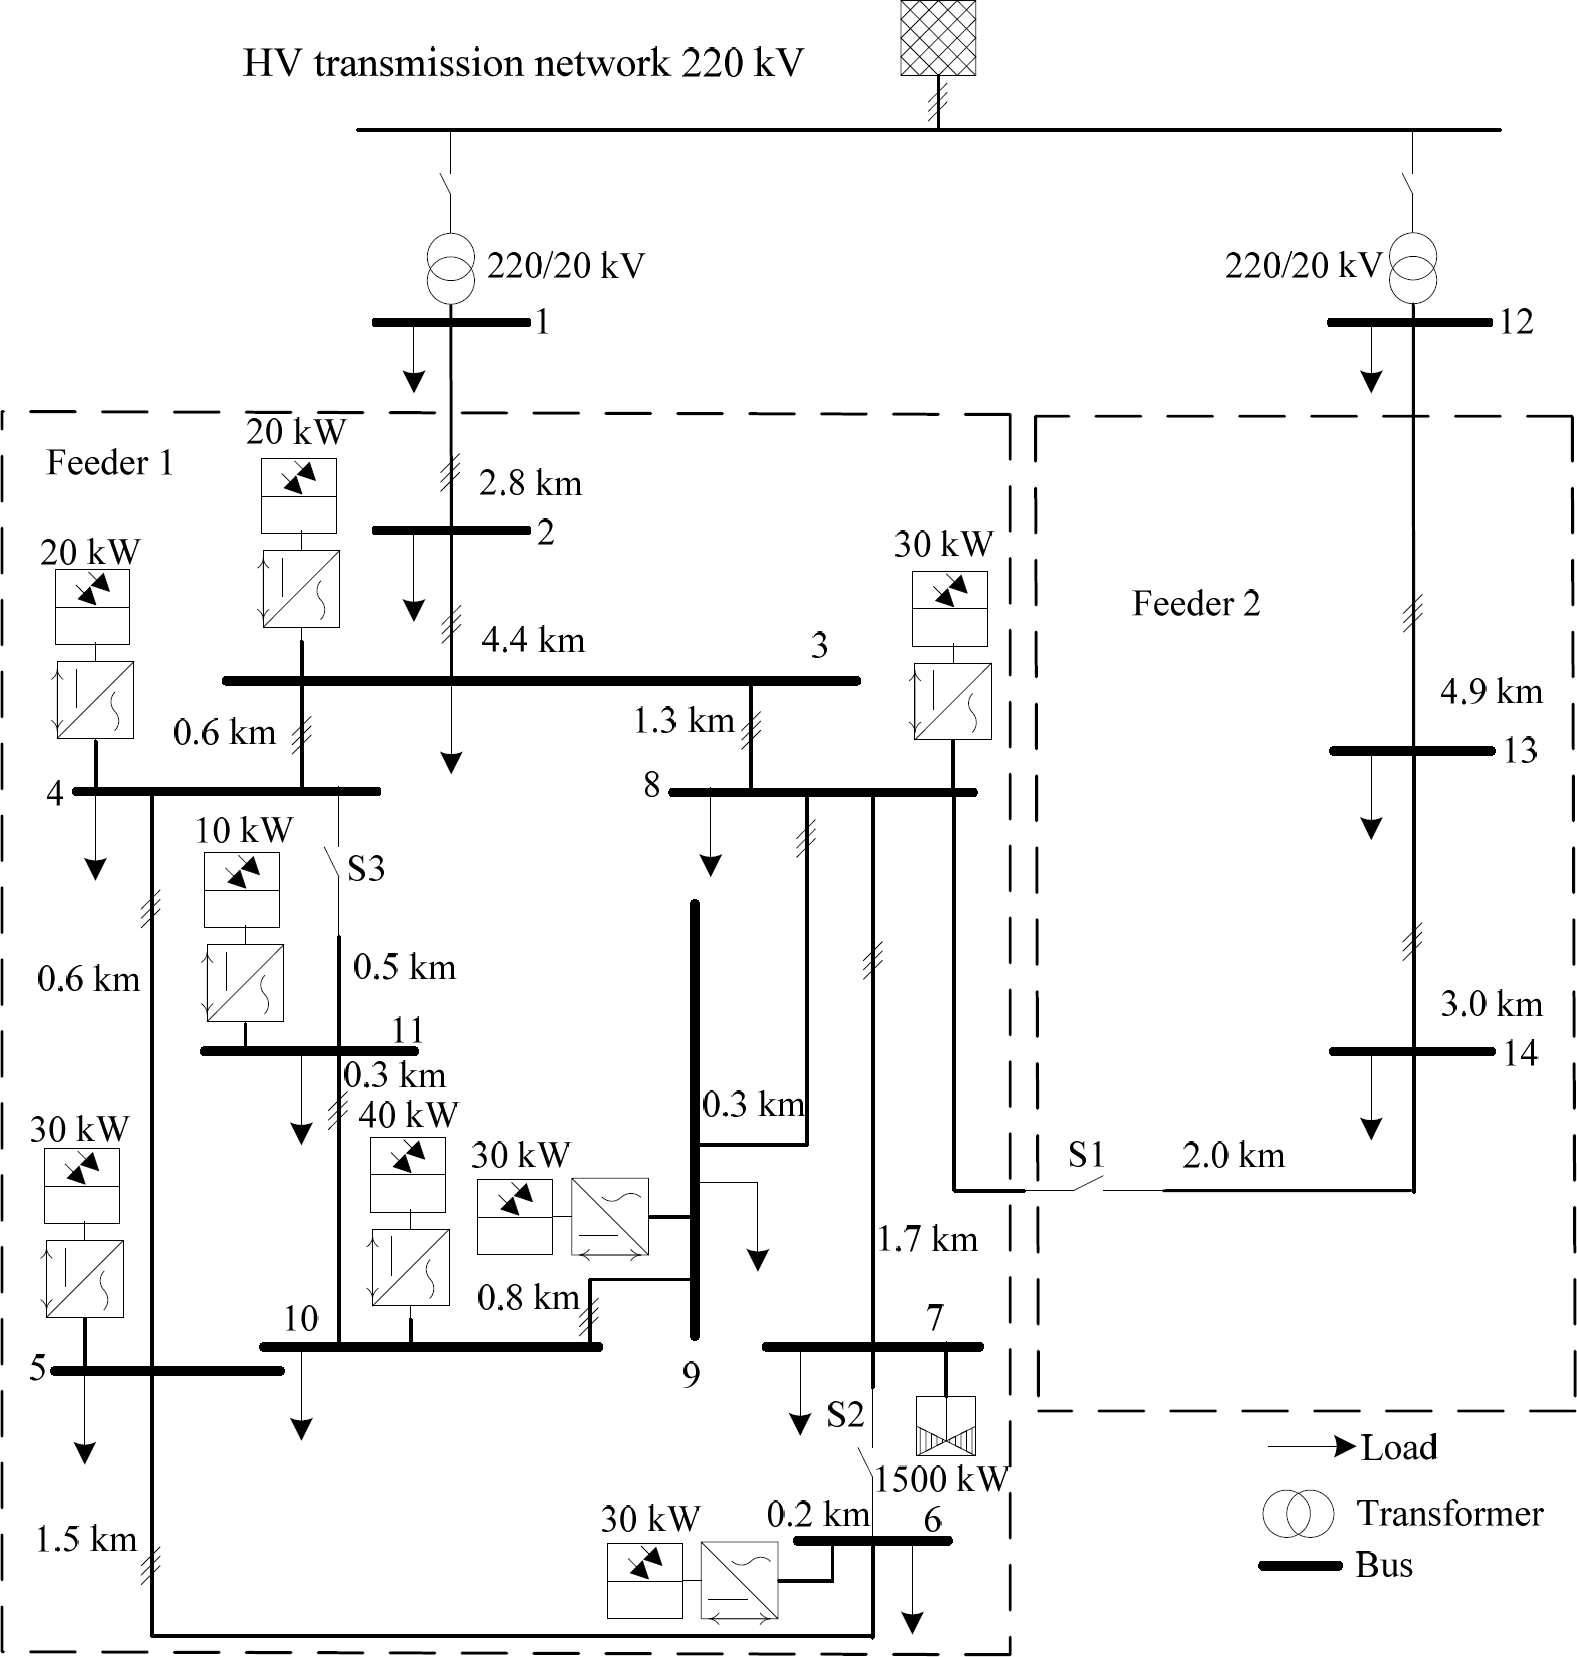
\includegraphics[height=14cm, width=13.5cm]{figures/cigre_network_mv_der.png}
    \caption[size = 9]{CIGRE network with solar and wind power that is used in the reinforcement learning algorithm}
    \label{fig:problem:cigre_network}
\end{figure}
The left-most feeder has several solar producing units connected and wind power connected to bus 7. The time resolution in this task is chosen to be hourly. In other words, the demand and solar production at every bus is updated every hour, and assumed constant in between hours. The demand profile is generated using \textit{enlopy}, a python toolkit for energy demand time series\cite{enlopy}. The demand signal is generated based on data of the energy consumption of private households. A data set with solar irradiance in Konongo, Ghana is used as input to define the production of solar power. The signal of solar production and power demand is assumed equal at all buses and scaled up based on nominal values of the loads at each bus. This reduces the state space, as there is no need for a unique demand forecast for all the loads.  For simplicity, the power factor is assumed constant at every bus, meaning the reactive power at each load is a percentage of the active power at all times. The power factor at each load is the same as the default values in the CIGRE network. The values of the solar production are intentionally amplified so that the safety margins for line current and voltage magnitudes in the grid frequently are violated if no actions are taken.  

All loads have an hourly forecast of energy consumption that is used to update the active and reactive powers at every time step. It is assumed that the loads at all buses have some flexibility, say 10 \% of the actual demand, that can be centrally controlled at every hour.

\section{Network variables}
The CIGRE network shown in figure \ref{fig:problem:cigre_network} is the power net the reinforcement algorithm is control. The number of components are summarised in table \ref{table:cigre_components}

\begin{table}[h]
\centering
\caption{Component in the CIGRE network}
\label{table:cigre_components}
\begin{tabular}{l|ll}

Component  & Symbol & Amount 
\\ 
\hline
Bus & N & 15 \\
Switch & - & 8 \\
Static generator &-& 9 \\ 
Line & - & 15 \\
Load &L & 18 \\
Transformer &- & 2

 \\
\hline
\end{tabular}
\end{table}
Only number of loads (\textit{L}) and number of buses \textit{B} is given since only they are relevant for describing reinforcement setup. Table \ref{table:cigre_components} shows that there are 18 loads and 15 buses in the system. The reason is that there are several loads connected to some buses which makes the number of loads greater than the number of buses.  



\section{State space}
It is not obvious how to design the state space for the agent. This section presents several spaces that could be useful for the reinforcement algorithm. Let $\mathcal{S}_{sun} \subseteq  \mathbb{R}^{k}$ be space of the forecasted total solar production in the grid \textit{k} hours into the future . This gives the agent information about the coming solar production in the power marked that can be used for finding strategies. For instance, consider a situation with a high production of solar power that is overreaching the capacity in the power lines. If the agent sees that there is a dip in solar production in the next hour due to clouds, it can increase the local demand at solar producing, to relieve the overloaded power lines. It can then safely decrease the demand the next hour, since the sun is blocked by the clouds. This is an example of a desired behaviour that the agent ideally should find. The buses are assumed to be geographically close, so the solar irradiance is the same. If a cloud blocks the sun at bus 1, then it also blocks the sun at all the other buses in the system. This significantly reduce the state space compared to a unique forecast for every bus. 


Let $\mathcal{S}_{demand} \subseteq \mathbb{R}^{k}$ be the space of the forecasted total demand in the grid $k$ hours into the future. The total demand in the market only partially describes the demand situations in the marked since the agent does not receive information about demand at individual loads. An advantage, however, is that the size of the a state vector from  $\mathcal{S}_{demand}$ is much smaller than a corresponding vector for all loads. Specifically, the CIGRE network that is used has 18 loads that would make the state vector 18 times greater.



Let $\mathcal{S}_{bus} \subseteq \mathbb{R}^{4N}$ be the space representing the state of all the buses in the net. Specifically

\begin{equation}
   \begin{aligned}
   \label{eq:problem:bus_state}
\mathcal{S}_{bus} = \{|V_{i}|, \delta_{i}, P_{i}, Q_{i} |\; i = 1,...,N\}
    \end{aligned} 
\end{equation}

where $|V_{i}|,\delta_{i}, P_{i}$ and $Q_{i}$ respectively are the voltage magnitude, voltage phase angle, active power injection and reactive power injection at bus $i$ in a $N$-bus system. This could give information to the agent about how stressed the system is. For instance, large values for active power $P_{i}$ and voltage magnitude $|V_{i}|$ indicate a stressed situation at bus $i$ possibly due to high solar production. 



The agent should also get information that ensures that the consumption at a load merely is shifted and not altered in absolute magnitude. In other words, a state that contains information about the energy balance in the grid. A positive energy balance means that the agent has forced the loads to use more energy than the real demand. If the agent changes a load by -1 MW for an hour, the agent should ideally increase the load by 1 MW some time not far into the future. Gemine et al did this by making a commitment when a load is modulated. When a load is modulated, it follows a predefined modulation curve for $T_{d}$ time steps (for instance 4 steps)\cite{active_network_management}. The modulation signal is constructed so that is sums to zero of over the time period $T_{d}$, which guarantees that the total energy consumption of the load is constant. This could be a possible approach for a reinforcement learning algorithm as well. The state vector could indicate in what modulation step a load is at. For instance, if the modulation started at $t_{0}$ for a load and the current time step is $t_{0} + 3$, then the load component of this vector is 3. The agent is then always fed with a signal that tells it the commitment stage of that load. The desired action of the agent at a time step in the commitment period will simply be ignored so that the load follows the modulation signal. This has the drawback that the agent's action frequently are overridden. Given a modulation period of \textit{k} steps, the agent desired action is only performed $1/k$ times. Hopefully the agent will pick up on this through the commitment state vector. Formally, the commitment space $\mathcal{S}_{commitment} \subseteq \mathbb{R}^{L}$ can be defined as



\begin{equation}
   \begin{aligned}
   \label{eq:problem:commitment_state}
\mathcal{S}_{commitment} = \{ c_{i} | i = 1,...,L\}
    \end{aligned} 
\end{equation}
where $c_{i} \in \{0,1,..,k\}$ is the commitment stage of load $i$ in a $k$-period commitment period in a grid with $L$ flexible loads. Table \ref{table:state_spaces} summarises the different state spaces. The reinforcement algorithm will be tested with several combinations of the spaces presented. In every case, the final state variable is constructed by concatenating the state vectors from different state spaces used. 

\begin{table}[h]
\centering
\caption{State spaces that can be used in the reinforcement algorithm. $H$ is the forecast horizon, i.e the number of hours into the future the agent receives a forecast. $N$ and $L$ are respectively the number of buses and flexible loads in the net. $r_{i}$ and $d_{i}$ are, respectively, the forecasted solar irradiance and power demand $i$ hour in the future. $|V_{i}|,\delta_{i}, P_{i}$ and $Q_{i}$ respectively are the voltage magnitude, voltage phase angle, active power injection and reactive power injection at bus $i$. $c_{i}$ is the commitment stage of flexible load \textit{i}}
\label{table:state_spaces}
\begin{tabular}{l|lll}

State space  & Symbol & Size & Definition
\\ 
\hline
Solar forecast      & $\mathcal{S}_{sun}$& H  &  $\{r_{i} |\;j=1,...,H\}$
\\ 

Demand forecast    & $\mathcal{S}_{demand}$ &$H\cdot L$ &$\{d_{j,i} |\;j=1,...,H,i=1,...,L\}$  \\ 
Bus state & $\mathcal{S}_{bus}$ & $4N$ &$\{\delta_{i}, P_{i}, Q_{i}, |V_{i}| |\; i = 1,...,N\}$\\

Commitment state &$\mathcal{S}_{commitment}$& $L$  &$\{ c_{i} |\; i = 1,...,L\}$ \\
  

\hline
\end{tabular}
\end{table}
\section{Action space}
The grid is controlled using demand response, which means that reinforcement agent can manipulate the active power demand at flexible loads in the power grid. The amount of flexibility at a load is defined to be certain percent of the real demand. It is assumed that the flexibility is symmetric so the demand can both be tuned up and down. The action space in a power grid with $L$ flexible load  $\mathcal{A}  \subseteq \mathbb{R}^{L}$ is defined as
\begin{equation}
   \begin{aligned}
   \label{eq:problem:action_space}
\mathcal{A}= \{a_{i} | i = 1,...,L\}
    \end{aligned} 
\end{equation}
where $a_{i} \in [-1,1]$ is the activation at flexible load $i$ in the power grid. $a_{i} = 1$ means that load $i$ increases its active power consumption as much as possible. The change in demand $\Delta P_{i}$ is then scaled up according to the action signal $a_{i}$ by

\begin{equation}
   \begin{aligned}
   \label{eq:problem:update_demand}
    \Delta P_{i}& = f_{i}P_{i}a_{i} \\
    P_{i}& \leftarrow P_{i} + \Delta P_{i}
    \end{aligned} 
\end{equation}
where $f_{i}$ is the flexibility at load, $P_{i}$ is the active power demand.

It is possible to include more control variables that the agent can control. For instance, the reinforcement agent could control the tap position of the transformer and the switches in the system. There is also a CIGRE benchmark network in pandapower that has storage units in the power net. A possible extension is to let the agent control the charging and discharging of storage units.

\section{Reward function}
A central element in any reinforcement algorithm is the reward function. The reward function should give a signal that is used to reinforce "good" behaviour. The goal of the agent is to not violate safety margins for voltage and current in the power grid. Gemine et al formulate a reward function aimed to safely operate a power grid at a low cost, where they punish the agent proportionally to the violation of safety margins\cite{active_network_management}. There are multiple cost terms that can be included, and this section will present several of these. 

There are safety margins in terms of voltage magnitudes in the power system. In the Norwegian power system this is between 0.95 and 1.05. In other word, Statnett tolerates a 5 \% deviation from nominal voltage in each direction. Let $C_{voltage,i}$ be the cost for violating voltage margins at bus $i$


\begin{equation}
   \begin{aligned}
   \label{eq:problem:voltage_margins_cost}
    C_{voltage,i} = max(0,|V_{i}| - V_{upper}) + max(0,V_{lower}- |V_{i}|)
    \end{aligned} 
\end{equation}
where $V_{upper}$ and $V_{lower}$ are the upper and lower per-unit voltage limit respectively. Let $C_{current,i}$ be the cost of violating current margins in line $i$

\begin{equation}
   \begin{aligned}
   \label{eq:problem:current_margins_cost}
    C_{current,i} = max(0,|I_{i}| - I_{upper})
    \end{aligned} 
\end{equation}
where $I_{upper}$ is the per unit upper current limit in lines. It is necessary to incentives costumers to offer flexibility in a realistic modelling of demand response. In other words, costumers should be economically compensated when their flexibility is activated. In classical incentive based programs (IBP) for demand control, costumers are given some sort of participation payment, such as a discount rate\cite{demand_response_definition}. On the other hand, marked based IBP compensates the costumers based on how much they participate. The most natural cost to consider in this thesis is the marked based IBP because the agent can is continuously change the consumption of power at flexible loads. The activation cost $C_{activation,i}$ is defined as

\begin{equation}
   \begin{aligned}
   \label{eq:problem:activation_cost}
    C_{activation,i} = \lambda \Delta P_{i}
    \end{aligned} 
\end{equation}
where $\Delta P_{i}$  is the change in demand at bus \textit{i} and $\lambda$ is the flexibility price at the time of activation.

\end{document}